This analysis lasted from September 12 - October 20, 2015 and contained a total
of 18.4 days of coincident detector data. After category 1 vetoes were applied, 17.9 days
of coincident data remained. After category 2 vetoes were applied, 17.8 days of coincident
data remained to be used in the final analysis. There were two interesting events that
occurred in this analysis period. The first is GW150914, a gravitational wave signal
from a binary black hole merger that marked the first direct detection of
gravitational waves\cite{GW150914-DETECTION}. The second is a marginal
detection candidate, LVT151012, which stands out
from the background distribution but does not have enough statistical
significance to be quoted as a confident detection.

The only major setting that was different between the analysis containing GW150914 
and the analysis containing GW151226 was the gating threshold. As discussed in 
Section \ref{sec:gating}, gating is used at the input to the search pipeline to 
remove large transients from the data before the analysis is run. 
For the analysis containing GW150914, Omicron 
was used to build the list of gating windows. A conservative threshold was set at Omicron SNR $>$ 300
to indicate a transient that should be gated. At each of these times a 1 second time window was constructed,
centered around the time of the transient, that indicated the stretch of data to be removed from the analysis.
This is the gating strategy that was employed in the analysis that included GW150914.
GW150914, which is considered to be a strong gravitational wave signal, was recovered by Omicron with an SNR
of 13 and 9 at Hanford and Livingston respectively, well beneath the gating threshold.

\section{BNS bin}

The BNS bin already has such clean statistics that it does not benefit from the
removal of data with excess noise.
Binary neutron star systems have the longest waveforms in the template bank, often spanning up
to 60 seconds in duration. With such long waveforms, the $\chi^{2}$ test is effective at
reducing the impact of transients on the BNS search. Typical instrumental transients have a small
number of cycles and a duration of less than 1 second. As such, the overlap between a transient
and a BNS signal is a small fraction of the total duration of the BNS waveform and is easily
distinguished as noise in the re-weighted SNR calculation. This is demonstrated in Figure
\ref{fig:bns-snr-newsnr}, which shows the distribution of single detector triggers in SNR
and re-weighted SNR. The tail of high SNR triggers is fully down-weighted, resulting in a
re-weighted SNR distribution that extends to $\hat{\rho} \approx 8.3$.

\begin{figure}[ht!]%
\centering
  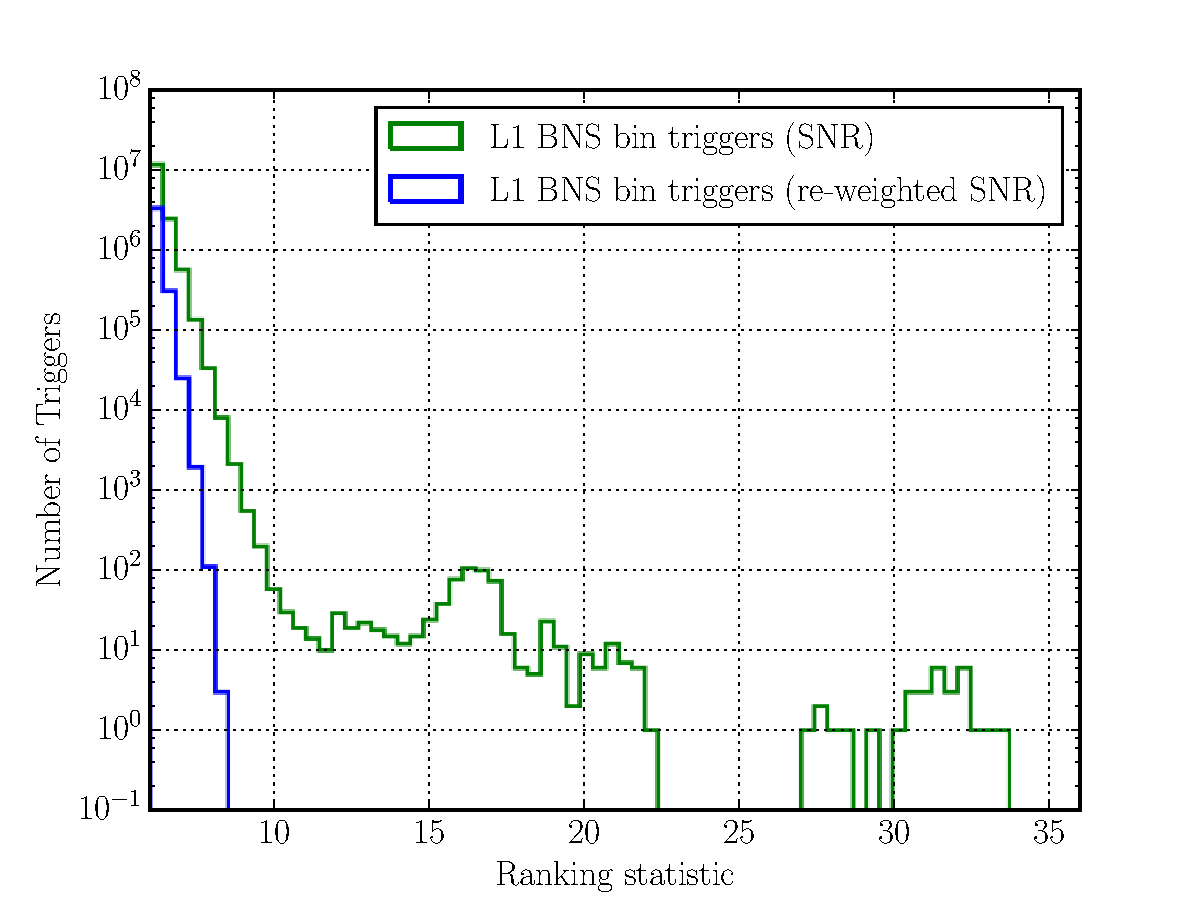
\includegraphics[width=0.8\textwidth]{figures/o1-cbc-dq-paper/bns-bin-newsnr-snr-comparison}
  \caption[Histogram of BNS bin triggers]{Histograms of Livingston (L1) single interferometer triggers found in the BNS bin. %
           The green curve shows the distribution of BNS bin triggers in SNR and the blue %
           curve shows the distribution of BNS bin triggers in %
           re-weighted SNR. The tail of high SNR triggers have all been down-weighted by the %
           $\chi^2$ test, leaving behind a re-weighted SNR distribution that has a shoulder %
           at just over $\hat{\rho} =$ 8. The total number of triggers in each histogram is %
           different, which is an artifact of the $\chi^2$ test down-weighting some triggers so %
           severely that they end up at $\hat{\rho} <$ 6. When the analysis is run, triggers %
           found with $\rho <$ 6 are discarded because of their low significance.}
  \label{fig:bns-snr-newsnr}
\end{figure}

Since the $\chi^{2}$ test is so effective in this bin, it is rare to see strong outliers in
the re-weighted SNR distribution.
Figure \ref{fig:bns-bin-far_GW150914} shows the background distribution of the BNS bin in the
PyCBC search for the analysis containing GW150914.
The cumulative rate of background events in a given bin
indicates the rate of false alarms expected in that bin for a given re-weighted SNR. In this bin,
there is no substantial improvement for any value of $\hat{\rho}_{c}$.
In both cases, the loudest background event is reported at $\hat{\rho}_{c} <$ 11.
The hypothetical detection candidate at $\hat{\rho}_{c} =$ 11.3 would be the loudest
event in this bin whether or not noisy data are removed. See Sections \ref{sec:bulk-bin} and
\ref{sec:edge-bin} for a contrary case.

\begin{figure}[!ht]%
\centering
  \subfloat[]{
  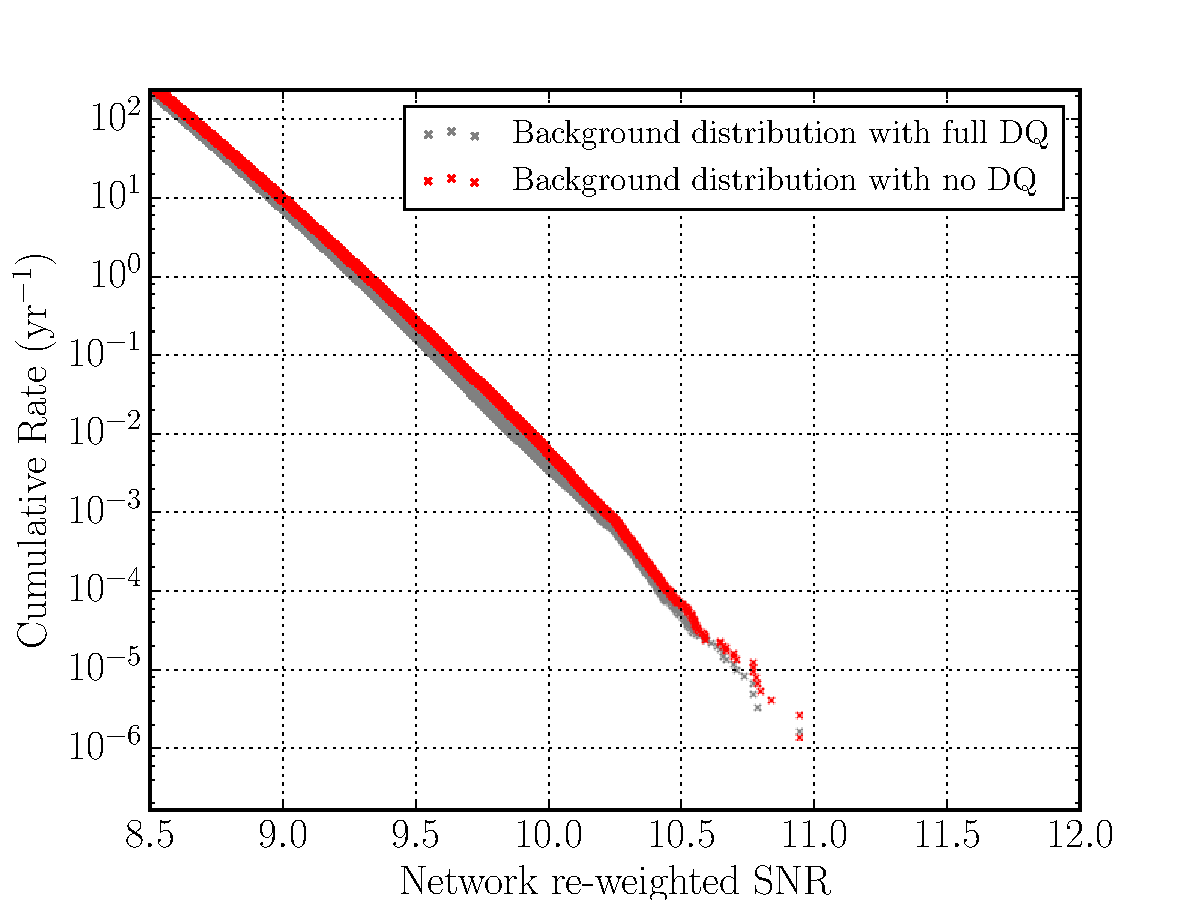
\includegraphics[width=0.495\textwidth]{figures/o1-cbc-dq-paper/bns_bin_far_GW150914}
  \label{subfig:bns-bin-gw150914-rate}
  }
  \subfloat[]{
  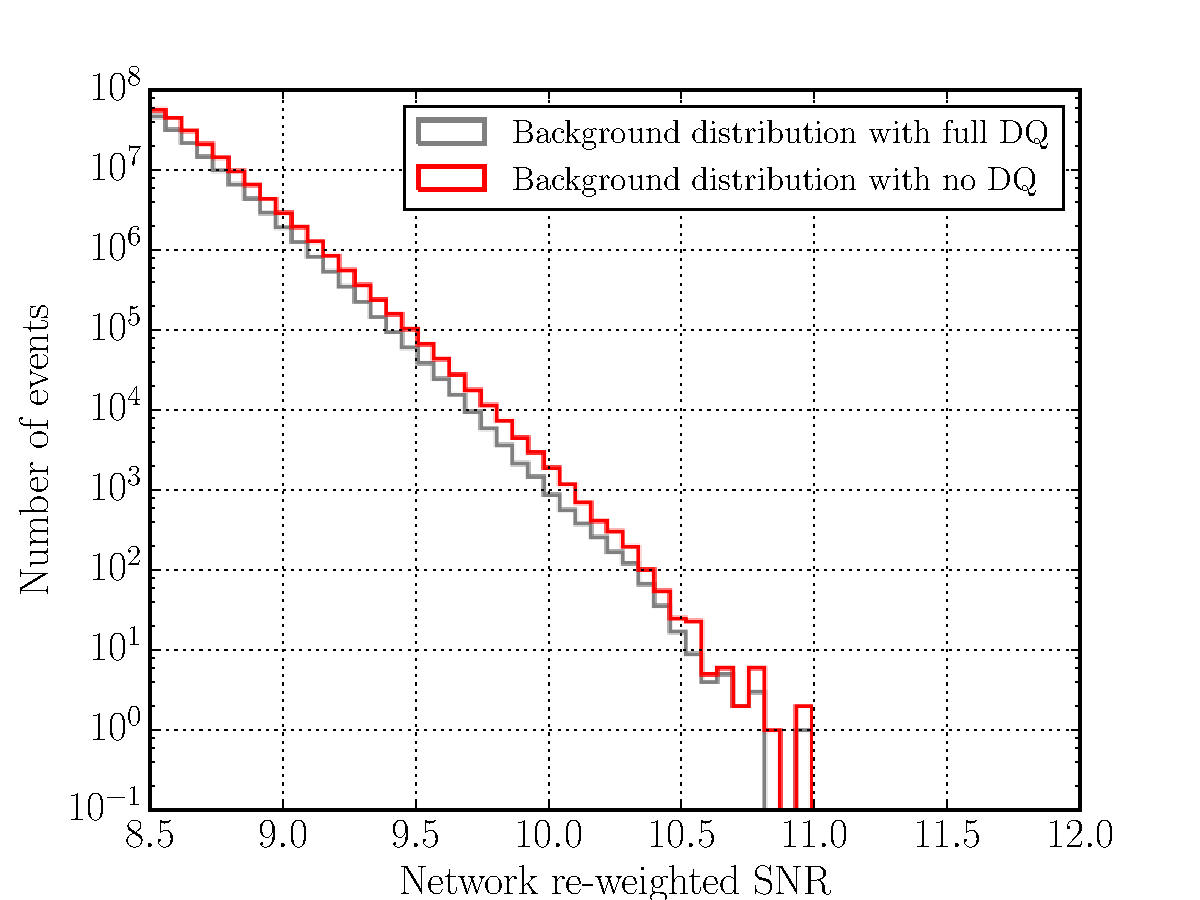
\includegraphics[width=0.495\textwidth]{figures/o1-cbc-dq-paper/bns_bin_GW150914_DQ_raw_hist}
  \label{subfig:bns-bin-gw150914-raw}
  }
  \caption[BNS bin histograms - GW150914 analysis]{The background distribution in the BNS bin before and after applying data quality (DQ) vetoes. %
           (\ref{subfig:bns-bin-gw150914-rate}) The cumulative rate of background triggers %
           in the BNS bin as a function of re-weighted SNR. %
           (\ref{subfig:bns-bin-gw150914-raw}) A histogram of background triggers %
           in the BNS bin. % 
           The red traces indicate the %
           distribution of background triggers without noisy data removed, %
           the gray traces indicate the distribution of background triggers with %
           all data quality vetoes applied. The BNS bin shows %
           minimal improvement in cumulative rate. A foreground event %
           at $\hat{\rho}_{c} =$ 11.3, representing the hypothetical detection %
           candidate, would be the loudest event in this bin.}
  \label{fig:bns-bin-far_GW150914}
\end{figure}

Table \ref{table:bns-far} shows the change in false alarm rate and probability at
$\hat{\rho}_c$ for multiple tiers
of data removal in the BNS bin. The false alarm rate and probability both decrease
if no data are removed from the analysis, indicating that the hypothetical detection candidate
appears more significant in the presence of noisy data. Since there are few loud triggers to be vetoed,
the overall effect of applying data quality vetoes is to reduce the overall analysis time, which
restricts the significance that can be assigned to a loud detection candidate.

\begin{table}[!ht]%
  \begin{center}
    \begin{tabular}{lcc}
      \hline
      Analysis configuration & False alarm rate ($\mathrm{yr}^{-1}$) & False alarm probability \\ \hline
      All vetoes applied & $1.65\times10^{-6}$ & $7.22\times10^{-8}$ \\
      No CAT2 applied & $1.63\times10^{-6}$ & $7.20\times10^{-8}$\\
      No CAT1 or CAT2 applied & $1.33\times10^{-6}$ & $6.50\times10^{-8}$\\
      \hline
    \end{tabular}
  \end{center}
  \caption[BNS bin FAR - GW150914 analysis]{Table of BNS bin false alarm rates and probabilities at $\hat{\rho}_{c} =$ 11.3 %
           for several analysis configurations. %
           Removing noisy data has a negligible effect on false alarm rates in the BNS bin. %
           The small differences in each configuration are due to data quality vetoes %
           changing the total amount of time used in background estimation.
           }
  \label{table:bns-far}
\end{table}

\section{Bulk bin}\label{sec:bulk-bin}

The bulk bin benefits much more from the application of data quality vetoes compared to the
BNS bin.
Figure \ref{fig:bulk-bin-far_GW150914} shows the background distribution in the bulk
bin for the analysis containing GW150914.
The
first noticeable change is that the loudest background event is at $\hat{\rho}_{c} =$
12.6 in the presence of noisy data compared to 11.5 when all data quality vetoes
are applied. This new loudest
event does not show up as a small outlier; there is a significant shoulder in the distribution that
persists up to $\hat{\rho}_{c} =$ 12 before falling off. Considering the two distributions as a whole,
there is a separation between the two curves beginning at $\hat{\rho}_{c} =$ 9, which reaches
an order of magnitude discrepancy at roughly $\hat{\rho}_{c} =$ 10 and continues to diverge at higher
values of network re-weighted SNR.

To quantify the difference between these two distributions, the hypothetical detection candidate at
$\hat{\rho}_{c} =$ 11.3 is
once again considered. In the analysis with noisy data removed, the hypothetical detection would be
amongst the loudest events in the distribution and with a false alarm rate of
$3.2\times10^{-6}$ as seen in Table \ref{table:bulk-far}. If data quality vetoes are
not applied,
the false alarm rate and false alarm probability increase by a factor of 1188,
severely diminishing the statistical significance of such an event.
Table \ref{table:bulk-far} also shows that the majority of the improvement in this bin
is the result of applying CAT1 vetoes. The difference between an analysis with all vetoes
applied and with CAT2 vetoes removed is negligible in the bulk bin.

\begin{figure}[!ht]%
\centering
  \subfloat[]{
  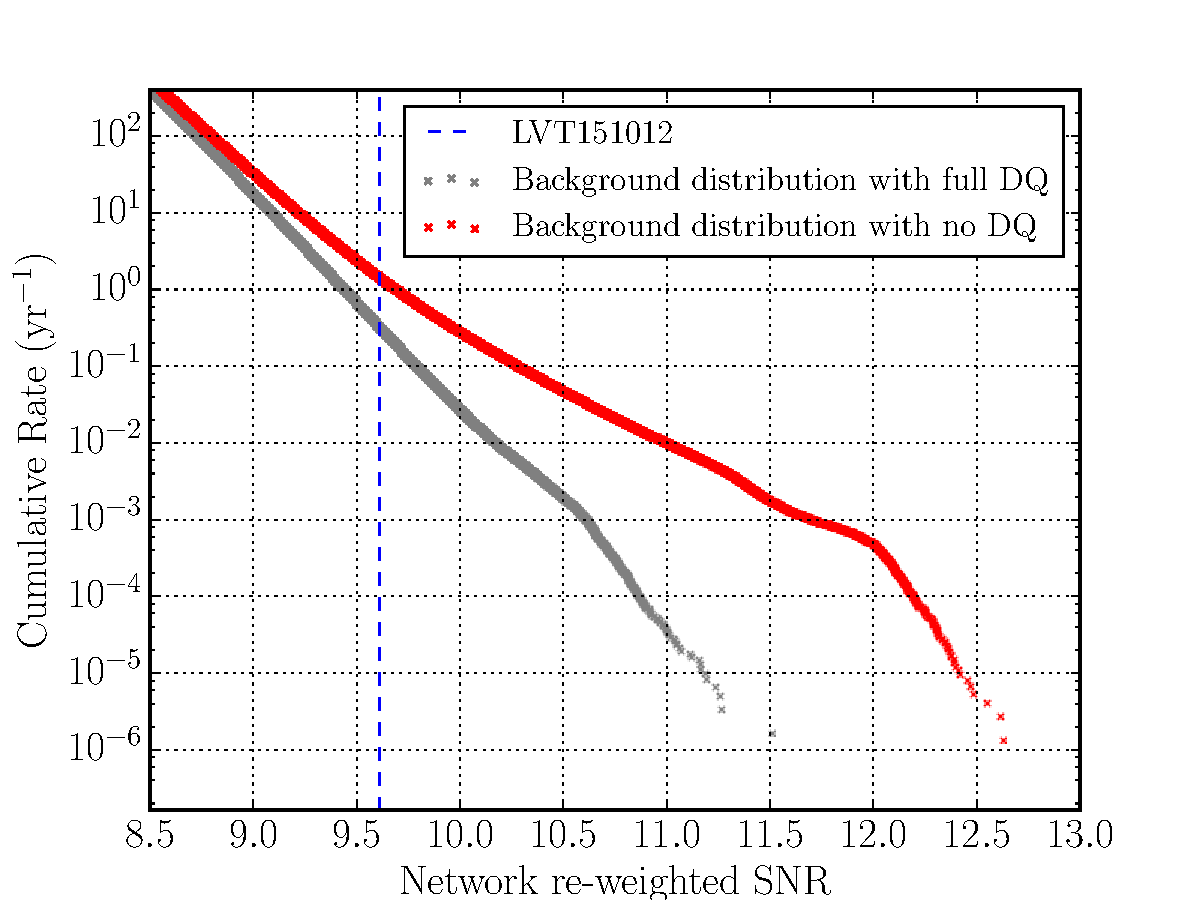
\includegraphics[width=0.495\textwidth]{figures/o1-cbc-dq-paper/bulk_bin_far_GW150914}
  \label{subfig:bulk-bin-gw150914-rate}
  }
  \subfloat[]{
  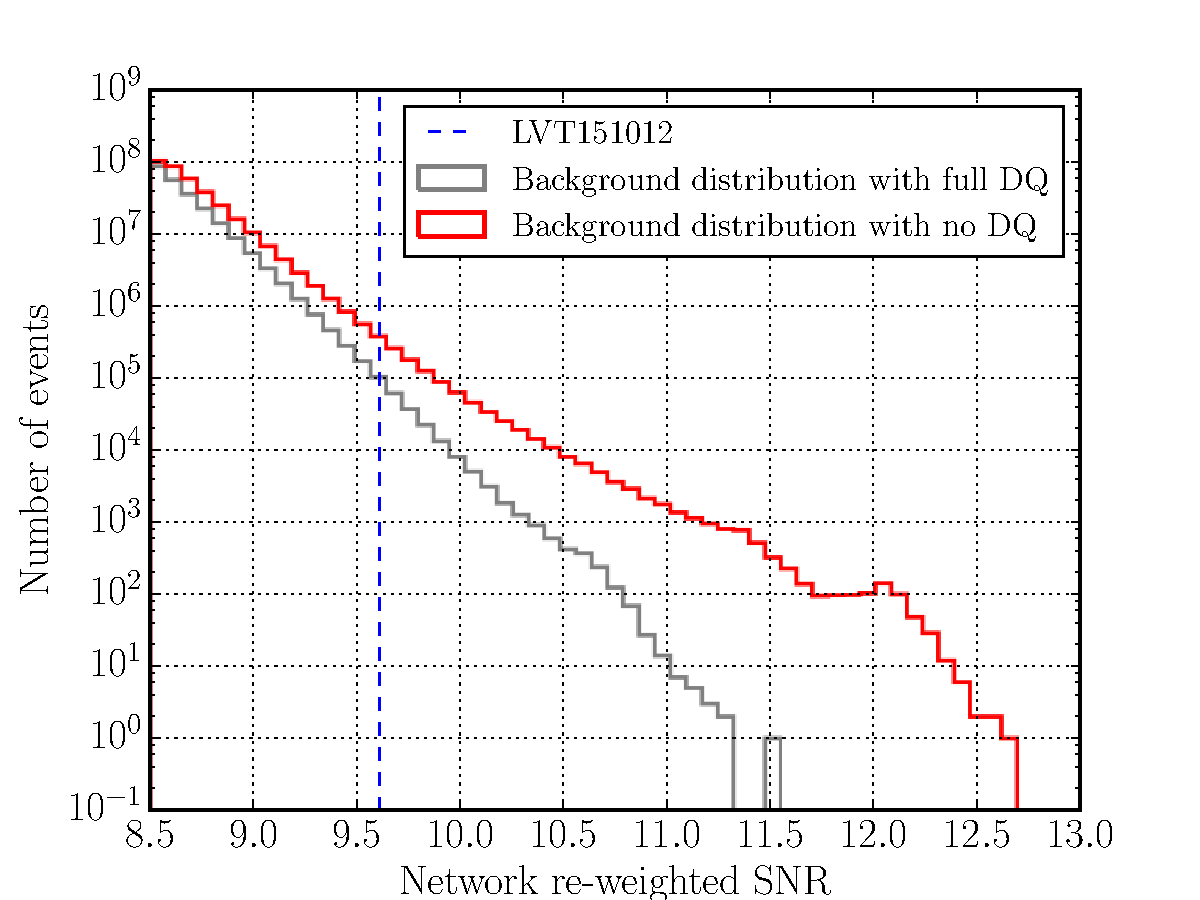
\includegraphics[width=0.495\textwidth]{figures/o1-cbc-dq-paper/bulk_bin_GW150914_raw_hist}
  \label{subfig:bulk-bin-gw150914-raw}
  }
  \caption[Bulk bin histograms - GW150914 analysis]{The background distribution in the bulk bin before and after applying data quality (DQ) vetoes. % 
           (\ref{subfig:bulk-bin-gw150914-rate}) The cumulative rate of background triggers %
           in the bulk bin as a function of re-weighted SNR. % 
           (\ref{subfig:bulk-bin-gw150914-raw}) A histogram of background triggers %
           in the bulk bin. %
           The red traces indicate the %
           distribution of background triggers without noisy data removed and the gray traces %
           indicate the distribution  %
           of background triggers with all data quality vetoes applied. The bulk bin sees %
           significant improvement when noisy data are removed, with over 3 orders %
           of magnitude of improvement at $\hat{\rho}_{c} =$ 11.3. The dotted line indicates the %
           network re-weighted SNR of LVT151012, an interesting candidate that was not %
           statistically significant enough to be claimed as a detection. The significance of %
           LVT151012 improved by a factor of 7.}
  \label{fig:bulk-bin-far_GW150914}
\end{figure}

\begin{table}[!ht]%
  \begin{center}
    \begin{tabular}{lcc}
      \hline
      Analysis configuration & False alarm rate ($\mathrm{yr}^{-1}$) & False alarm probability \\ \hline
      All vetoes applied & $3.29\times10^{-6}$ & $1.44\times10^{-7}$\\
      No CAT2 applied & $3.27\times10^{-6}$ & $1.44\times10^{-7}$ \\
      No CAT1 or CAT2 applied & $3.91\times10^{-3}$ & $1.91\times10^{-4}$ \\
      \hline
    \end{tabular}
  \end{center}
  \caption[Bulk bin FAR - GW150914 analysis]{Table of bulk bin false alarm rates and probabilities at $\hat{\rho}_{c} =$ 11.3 %
           for several analysis configurations. %
           The effects of removing data with excess noise are considerable in the %
           bulk bin. The hypothetical detection candidate %
           shows over 3 orders of magnitude of improvement in false alarm rate
           when all vetoes have been applied.
           }
  \label{table:bulk-far}
\end{table}

\subsection{LVT151012}\label{sec:LVT151012}
The second most significant trigger in the analysis containing GW150914 was LVT151012,
recorded on October 12, 2015.
The trigger was recovered in the bulk bin with $\hat{\rho}_{c} =$ 9.6, which lies in the region
where data quality vetoes are expected to begin having a significant impact on false alarm rates,
as discussed in Chapter \ref{ch:Vetoes}.

LVT151012 provides an interesting test case for this study. It had a
false alarm probability of 2\%, making it an interesting candidate but not
statistically significant enough to be claimed as a detection. Though slightly quieter, it is
analagous
to the hypothetical detection candidate considered in Chapter \ref{ch:Vetoes}.

The application of data quality vetoes increased the significance of LVT151012.
The false alarm rate and probability both decrease by a factor of 7 when data quality vetoes are
applied, as shown in Table \ref{table:151012-far}.

\begin{table}[!ht]%
  \begin{center}
    \begin{tabular}{lcc}
      \hline
      Analysis configuration & False alarm rate ($\mathrm{yr}^{-1}$) & False alarm probability \\ \hline
      All vetoes applied & $0.44$ & $2.03\times10^{-2}$ \\
      No CAT2 applied & $0.51$ & $2.35\times10^{-2}$ \\
      No CAT1 or CAT2 applied & $3.09$ & $0.14$ \\
      \hline
    \end{tabular}
  \end{center}
  \caption[LVT150914 FAR]{Table of bulk bin false alarm rates and probabilities for LVT151012 using several %
           different analysis %
           configurations. The false alarm rate and probability of LVT151012 were reduced by a %
           factor of 7 when noisy data were removed from the analysis.}
  \label{table:151012-far}
\end{table}

\section{Edge bin}\label{sec:edge-bin}

The edge bin is significantly impacted by the application of data quality vetoes, although in a
different way than the bulk bin. Figure \ref{fig:edge-bin-far_GW150914} shows the background
distribution in the edge bin before and after data with excess noise have been removed from the analysis.
If noisy data are not removed from the analysis, there is
a noticeable extension of the tail of loudest events. The loudest background event with no data
removed from the analysis is at $\hat{\rho}_{c} =$ 19.3 compared to $\hat{\rho}_{c} =$ 13.3
when all vetoes are applied.
When data with excess noise is removed, any trigger with $\hat{\rho}_{c} >$ 13.3 would be the loudest event in
the analysis
with a false alarm rate of O$(10^{-6} \mathrm{yr}^{-1})$. When no data are removed, the region between
$\hat{\rho}_{c} =$ 13.3 and
$\hat{\rho}_{c} =$ 18 is constrained to a false alarm rate of O$(10^{-3} \mathrm{yr}^{-1})$ due to the long
tail of background triggers.

\begin{figure}[!ht]%
\centering
  \subfloat[]{
  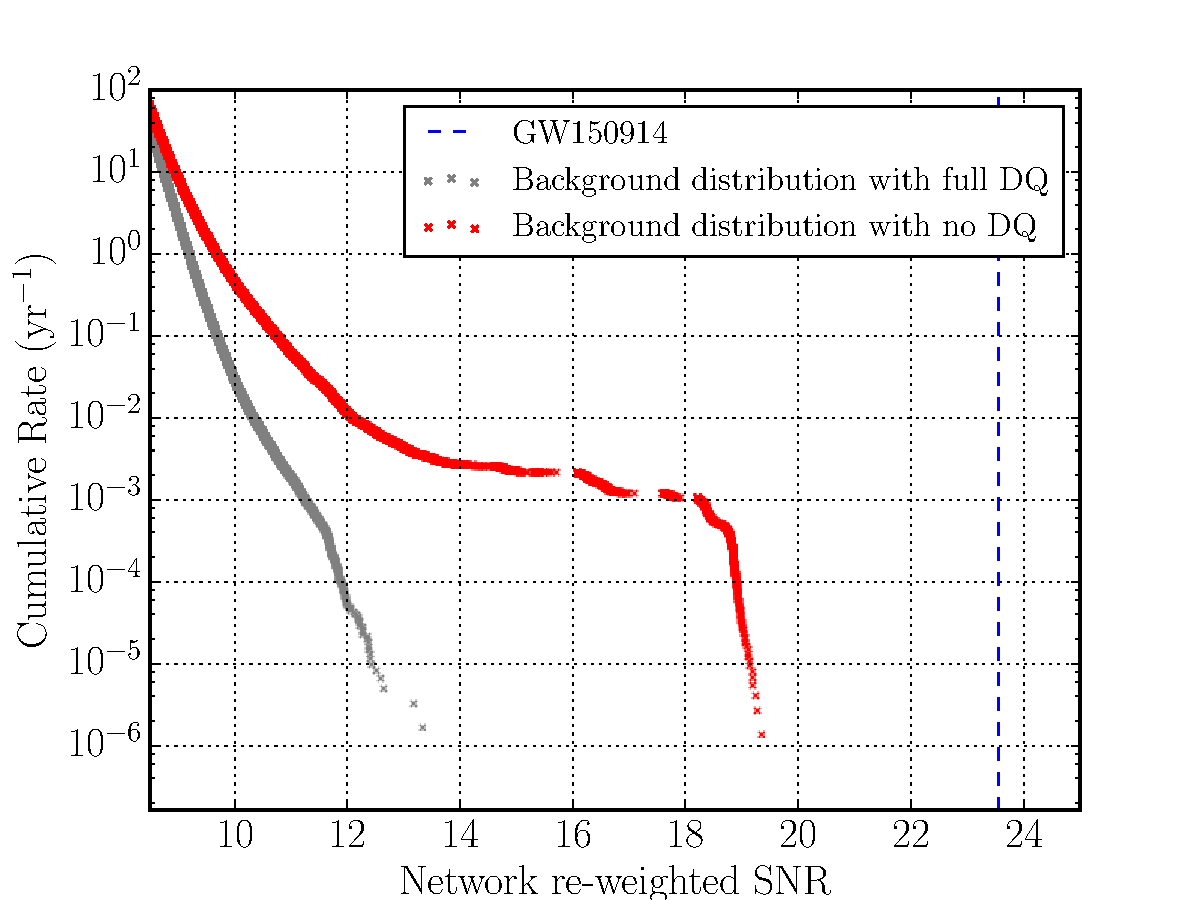
\includegraphics[width=0.495\textwidth]{figures/o1-cbc-dq-paper/edge_bin_far_GW150914}
  \label{subfig:edge-bin-gw150914-rate}
  }
  \subfloat[]{
  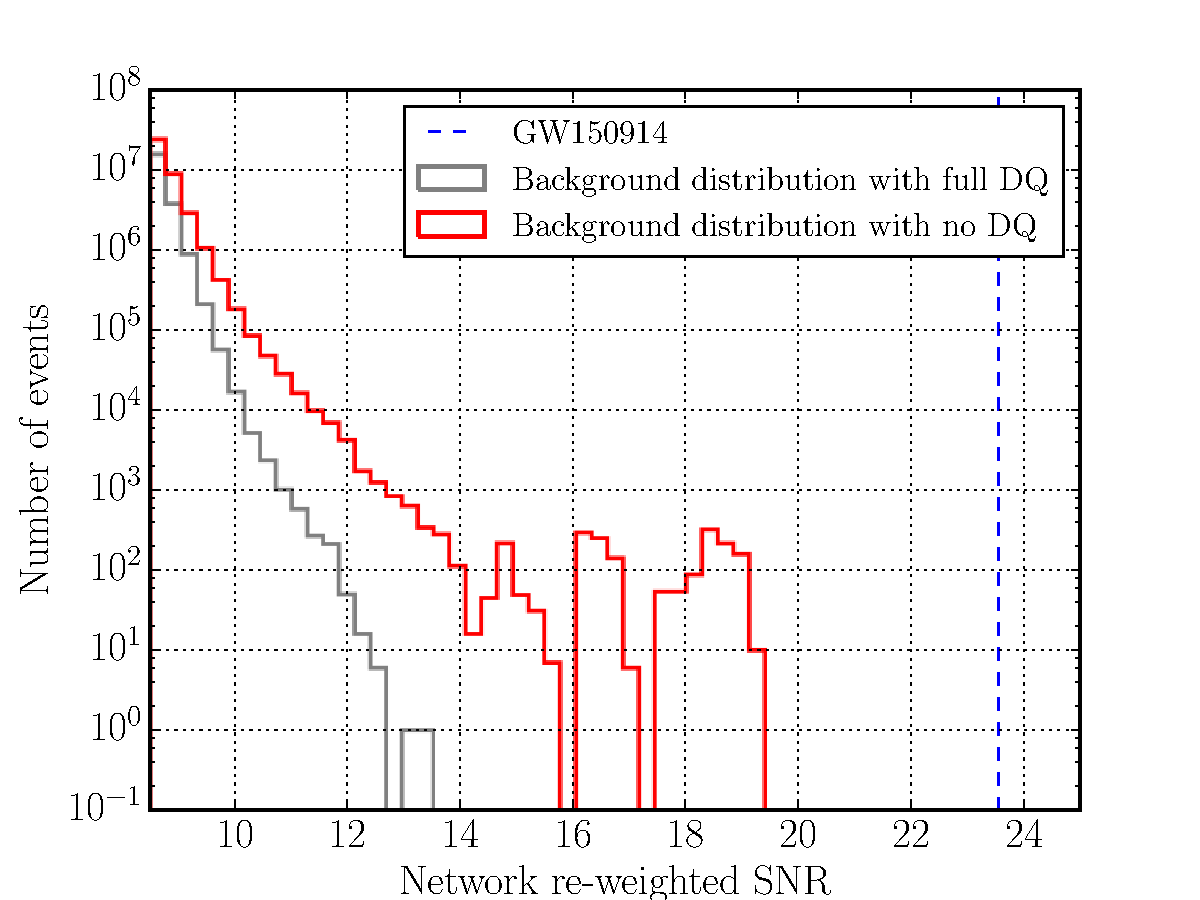
\includegraphics[width=0.495\textwidth]{figures/o1-cbc-dq-paper/edge_bin_GW150914_DQ_raw_hist}
  \label{subfig:edge-bin-gw150914-raw}
  }
  \caption[Edge bin histograms - GW150914 analysis]{The background distribution in the edge bin before and after applying data quality (DQ) vetoes. %
           (\ref{subfig:edge-bin-gw150914-rate}) The cumulative rate of background triggers %
           in the edge bin as a function of re-weighted SNR. %
           (\ref{subfig:edge-bin-gw150914-raw}) A histogram of background triggers %
           in the edge bin. % 
           The red traces indicate the %
           distribution of background triggers without noisy data removed from the analysis and %
           the gray traces indicate the distribution of background triggers with all data % 
           quality vetoes applied. %
           The dotted line indicates GW150914, which was recovered with $\hat{\rho}_{c} =$ 23.56. %
           When noisy data are not removed, the tail of the distribution extends to $\hat{\rho}_{c} =$ 19.5, %
           which severely impacts the ability to make a significant detection in the %
           $\hat{\rho}_{c} >$ 13.3 region. In both cases, GW150914 is the loudest event %
           in this bin.
          }
\label{fig:edge-bin-far_GW150914}
\end{figure}

Consideration of the hypothetical detection candidate at $\hat{\rho}_{c} =$ 11.3 reveals an
order of magnitude improvement
in false alarm rate and probability when data quality vetoes are used to remove data.
This is not as dramatic as
the improvement shown in the bulk bin, but it is still significant. This improvement is
quantified in Table \ref{table:edge-far}. It is interesting to note
that both the bulk and the edge begin to show improvement around $\hat{\rho}_{c} =$ 9 and
show very similar levels
of improvement at $\hat{\rho}_{c} =$ 10, but their behavior begins to diverge after this point.

\begin{table}[!ht]%
  \begin{center}
    \begin{tabular}{lcc}
      \hline
      Analysis configuration & False alarm rate ($\mathrm{yr}^{-1}$) & False alarm probability \\ \hline
      All vetoes applied & $9.13\times10^{-4}$ & $4.00\times10^{-5}$ \\
      No CAT2 applied & $2.24\times10^{-3}$ & $9.84\times10^{-5}$ \\
      No CAT1 or CAT2 applied & $3.74\times10^{-2}$ & $1.82\times10^{-3}$ \\
      \hline
    \end{tabular}
  \end{center}
  \caption[Edge bin FAR - GW150914 analysis]{Table of edge bin false alarm rates and probabilities at $\hat{\rho}_{c} =$ 11.3 %
           for several analysis configurations. %
           The false alarm rate is decreased when noisy data are removed, %
           resulting in a factor of 40 improvement when data quality are applied. CAT2 vetoes have a %
           greater impact in this bin, though they are still not as impactful as CAT1.}
  \label{table:edge-far}
\end{table}

\subsection{GW150914}

The gravitational wave signal GW150914, produced from the inspiral and merger of a binary black
hole system, was detected on September 14, 2015 and was recovered by the PyCBC search with
$\hat{\rho}_{c} =$ 23.6 \cite{GW150914-DETECTION}.
GW150914 was louder than
any background event in the analysis regardless of what data were considered. This being
the case, data quality vetoes do not improve the false alarm rate for GW150914. It should be
noted that GW150914 was an exceptionally loud event that sits well above the search background
and is not the type of event that is expected to benefit from data quality vetoes.
This is quantified in Table \ref{table:150914-far}.

\begin{table}[!ht]%
  \begin{center}
    \begin{tabular}{lcc}
      \hline
      Analysis configuration & False alarm rate ($\mathrm{yr}^{-1}$) & False alarm probability \\ \hline
      All vetoes applied & $4.94\times10^{-6}$ & $2.17\times10^{-7}$ \\
      No CAT2 applied & $4.90\times10^{-6}$ & $2.16\times10^{-7}$ \\
      No CAT1 or CAT2 applied & $3.99\times10^{-6}$ & $1.95\times10^{-7}$ \\
      \hline
    \end{tabular}
  \end{center}
  \caption[GW150914 FAR]{Table of edge bin false alarm rates and probabilities for GW150914 for several analysis %
           configurations. GW150914 is loud enough that its false alarm probability %
           is not strongly affected by removing noisy data from the analysis. The slight change seen %
           in each column is due to each analysis configuration allowing different amounts of %
           analysis time. %
           }
  \label{table:150914-far}
\end{table}

